% =====================================================================
%  MCMP117 -- Fundamentals of Operating Systems
%  Week 1 Course Notes: The Big Picture & a History of Computing
%  Compile with XeLaTeX (twice, for references):
%      xelatex MCMP117_Week1_Notes.tex
%      xelatex MCMP117_Week1_Notes.tex
%  Images are expected in ./figures/
% =====================================================================
\documentclass[11pt,a4paper]{article}

% ---------- Page & fonts ---------------------------------------------
\usepackage[a4paper,margin=2.3cm,headheight=15pt]{geometry}
\usepackage{fontspec}
\IfFontExistsTF{Calibri}{\setmainfont{Calibri}}{\setmainfont{Carlito}}
\IfFontExistsTF{Cambria}{\newfontfamily\headfont{Cambria}}{\newfontfamily\headfont{Caladea}}
\IfFontExistsTF{Consolas}{\setmonofont[Scale=0.95]{Consolas}}{\setmonofont[Scale=0.88]{DejaVu Sans Mono}}
\usepackage{amsmath,amssymb}
\usepackage{microtype}
\linespread{1.12}
\setlength{\parskip}{0.55em}
\setlength{\parindent}{0pt}

% ---------- Colours (course design system) ----------------------------
\usepackage{xcolor}
\definecolor{dark}{HTML}{212121}
\definecolor{charcoal}{HTML}{36454F}
\definecolor{slate}{HTML}{50808E}
\definecolor{mint}{HTML}{02C39A}
\definecolor{mintdeep}{HTML}{028090}
\definecolor{light}{HTML}{F2F2F2}
\definecolor{muted}{HTML}{6B7679}

% ---------- Packages ---------------------------------------------------
\usepackage{graphicx}
\usepackage{float}
\usepackage{needspace}
\graphicspath{{figures/}}
\usepackage[font=small,labelfont={bf,color=mintdeep},justification=centering]{caption}
\usepackage{booktabs,longtable,array,tabularx}
\usepackage{enumitem}
\setlist{itemsep=0.25em,topsep=0.3em}
\usepackage{tikz}
\usetikzlibrary{arrows.meta,positioning,calc,shapes.geometric}
\usepackage{pgfplots}
\pgfplotsset{compat=1.17}
\usepackage[most]{tcolorbox}
\usepackage{titlesec}
\usepackage{fancyhdr}
\usepackage{xurl}
\usepackage[colorlinks=true,linkcolor=mintdeep,urlcolor=mintdeep,citecolor=mintdeep]{hyperref}

% ---------- Headings ----------------------------------------------------
\titleformat{\section}{\headfont\Large\bfseries\color{charcoal}}{\color{mint}\thesection}{0.7em}{}
\titleformat{\subsection}{\headfont\large\bfseries\color{charcoal}}{\color{mintdeep}\thesubsection}{0.6em}{}
\titleformat{\subsubsection}{\headfont\normalsize\bfseries\color{mintdeep}}{}{0em}{}
\titlespacing*{\section}{0pt}{1.6em}{0.6em}
\titlespacing*{\subsection}{0pt}{1.2em}{0.4em}

% ---------- Header / footer -----------------------------------------------
\pagestyle{fancy}
\fancyhf{}
\fancyhead[L]{\small\color{muted}MCMP117 --- Fundamentals of Operating Systems}
\fancyhead[R]{\small\color{muted}Week 1 Notes}
\fancyfoot[C]{\small\color{muted}\thepage}
\renewcommand{\headrulewidth}{0pt}

% ---------- Boxes ---------------------------------------------------------
\newtcolorbox{keyidea}[1][Key idea]{enhanced,breakable,colback=charcoal,colframe=charcoal,
  coltext=white,fonttitle=\headfont\bfseries\color{mint},title={#1},
  attach title to upper={\par\smallskip},boxrule=0pt,arc=3pt,left=10pt,right=10pt,top=8pt,bottom=8pt}
\newtcolorbox{example}[1][Worked example]{enhanced,colback=light,colframe=light,
  fonttitle=\headfont\bfseries\color{mintdeep},title={#1},attach title to upper={\par\smallskip},
  boxrule=0pt,arc=3pt,left=10pt,right=10pt,top=8pt,bottom=8pt}
\newtcolorbox{tryit}[1][Try it yourself]{enhanced,breakable,colback=white,colframe=mint,
  fonttitle=\headfont\bfseries\color{mintdeep},title={#1},attach title to upper={\par\smallskip},
  boxrule=0.8pt,arc=3pt,left=10pt,right=10pt,top=8pt,bottom=8pt}
\newtcolorbox{histnote}[1][Historical note]{enhanced,breakable,colback=white,colframe=slate!40,
  fonttitle=\headfont\bfseries\color{slate},title={#1},attach title to upper={\par\smallskip},
  boxrule=0.5pt,arc=3pt,left=10pt,right=10pt,top=8pt,bottom=8pt,fontupper=\small}

% Photo helper: fits image inside a box, never distorted (keepaspectratio)
\newcommand{\photo}[3]{\includegraphics[width=#1,height=#2,keepaspectratio]{#3}}

\newcommand{\term}[1]{\textbf{\color{mintdeep}#1}}
\newcommand{\cmd}[1]{\texttt{#1}}

% =====================================================================
\begin{document}

% ---------------------------- Title block ------------------------------
\thispagestyle{empty}
\begin{tcolorbox}[enhanced,colback=dark,colframe=dark,arc=0pt,boxrule=0pt,
  left=18pt,right=18pt,top=20pt,bottom=20pt,coltext=white]
{\small\color{mint}\textsc{MCMP117 \,·\, Week 1 \,·\, Course Notes}}\par\medskip
{\headfont\fontsize{26}{30}\selectfont\bfseries Fundamentals of Operating Systems}\par\medskip
{\large The Big Picture \& a History of Computing}\par\smallskip
{\small\itshape\color{white!70} What is a computer? What is an operating system? And how did we get here?}
\end{tcolorbox}

\vspace{0.4em}
{\small
\textbf{Instructor:} Asst.\ Prof.\ Dr.\ (Ph.D.) Hasan Oğuz\\
Head of the Electronical Communication Technology Programme, Vocational School\\
Istanbul Okan University\par}

\vspace{0.8em}
\begin{keyidea}[What you should be able to do after this week]
\begin{enumerate}[leftmargin=1.4em]
  \item Describe a computer as a machine that follows instructions, using the \emph{input $\to$ process $\to$ output} model.
  \item Give a first, working definition of an operating system (OS) and explain three things it does.
  \item Explain \emph{why} we need an OS, by comparing a computer with and without one.
  \item Place the major milestones of computing history on a timeline, from Babbage's Analytical Engine to cloud computing.
  \item Explain, with a simple calculation, why ideas such as \emph{batch processing}, \emph{multiprogramming} and \emph{time-sharing} were invented.
\end{enumerate}
\end{keyidea}

\setcounter{tocdepth}{2}
\tableofcontents

% =====================================================================
\section{What Is a Computer, Really?}

Strip away the screen, the keyboard and the apps. At its core, a \term{computer} is a machine that \emph{follows instructions}. It takes some \emph{input}, \emph{processes} it according to a list of instructions (a \term{program}), and produces an \emph{output}.

\begin{figure}[H]
\centering
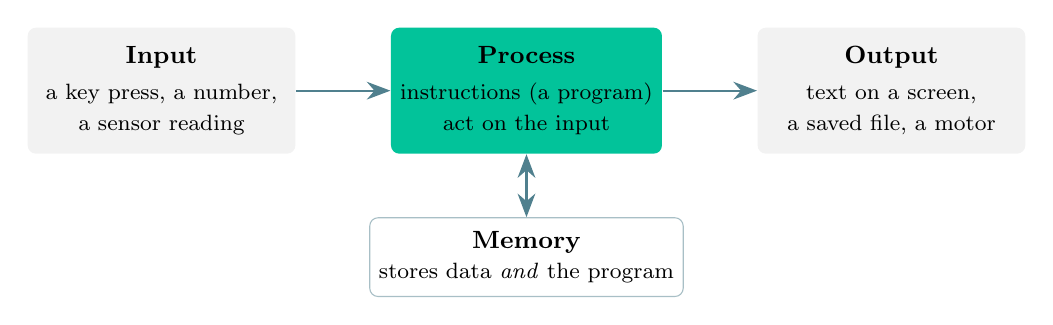
\begin{tikzpicture}[
  box/.style={rectangle,rounded corners=3pt,minimum width=3.4cm,minimum height=1.6cm,align=center,font=\small},
  arr/.style={-{Stealth[length=3mm]},thick,color=slate}]
\node[box,fill=light] (in) {\headfont\bfseries Input\\[2pt]\footnotesize a key press, a number,\\\footnotesize a sensor reading};
\node[box,fill=mint,right=1.2cm of in] (pr) {\headfont\bfseries Process\\[2pt]\footnotesize instructions (a program)\\\footnotesize act on the input};
\node[box,fill=light,right=1.2cm of pr] (out) {\headfont\bfseries Output\\[2pt]\footnotesize text on a screen,\\\footnotesize a saved file, a motor};
\draw[arr] (in) -- (pr);
\draw[arr] (pr) -- (out);
\node[box,fill=white,draw=slate!50,minimum width=3.4cm,minimum height=1.0cm,below=0.8cm of pr] (mem) {\headfont\bfseries Memory\\\footnotesize stores data \emph{and} the program};
\draw[arr,{Stealth[length=3mm]}-{Stealth[length=3mm]}] (pr) -- (mem);
\end{tikzpicture}
\caption{The input--process--output (IPO) model. Memory holds both the data and the program itself.}
\label{fig:ipo}
\end{figure}

Two details in Figure~\ref{fig:ipo} matter for the rest of the course:

\begin{itemize}
  \item \textbf{The program is stored in memory, just like data.} This is called the \term{stored-program} idea. It means we can change what the computer does simply by loading a different program, with no rewiring. As we will see in Section~\ref{sec:gen1}, the very first electronic computers did \emph{not} work this way.
  \item \textbf{The loop never stops.} The processor repeats the same cycle: \emph{fetch} the next instruction from memory, \emph{decode} it, \emph{execute} it. A modern processor does this billions of times per second.
\end{itemize}

\begin{example}[How fast is ``billions of times per second''?]
A processor running at a clock frequency of $f = 3\ \text{GHz}$ completes one clock cycle in
\[
T = \frac{1}{f} = \frac{1}{3\times 10^{9}\ \text{s}^{-1}} \approx 0.33\ \text{ns}.
\]
In that time, light travels only about $c\,T \approx (3\times10^{8}\ \text{m/s})(0.33\times10^{-9}\ \text{s}) \approx 10\ \text{cm}$. Waiting even $10\ \text{ms}$ for a hard disk therefore costs about $3\times10^{7}$ clock cycles. Keep this number in mind: most of operating-system history is about \emph{not wasting} those cycles.
\end{example}

Every computer you will ever meet follows this same loop, whether it is a phone, a laptop, a drone's flight controller or a washing machine.

% =====================================================================
\section{What Is an Operating System?}

\begin{keyidea}[A first definition (we will sharpen it in Week 2)]
The \textbf{operating system} is the program that starts first when you turn the computer on, and that manages everything else, so that other programs can run.
\end{keyidea}

This short definition hides three separate jobs:

\begin{enumerate}[leftmargin=1.4em]
  \item \textbf{It starts first.} When you press the power button, a small piece of firmware checks the hardware and then loads the OS. Every other program, whether your browser, a game or a text editor, is started \emph{by} the OS.
  \item \textbf{It manages everything else.} Many programs want the processor, the memory, the disk and the network at the same time. The OS decides who gets what, and when.
  \item \textbf{It hides the hard parts.} You press \emph{Save}; you do not need to know which sectors of which disk your file lands on. The OS offers simple, uniform services in place of complicated hardware details.
\end{enumerate}

\begin{figure}[H]
\centering
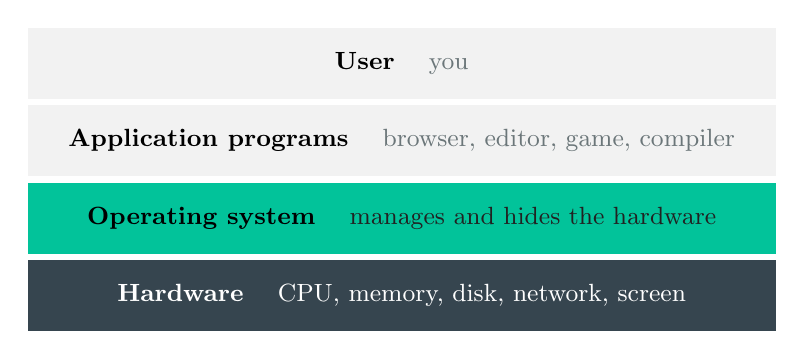
\begin{tikzpicture}[layer/.style={rectangle,minimum width=9.5cm,minimum height=0.9cm,align=center,font=\small}]
\node[layer,fill=light] (u) {\textbf{User} \quad {\color{muted}you}};
\node[layer,fill=light,below=2pt of u] (a) {\textbf{Application programs} \quad {\color{muted}browser, editor, game, compiler}};
\node[layer,fill=mint,below=2pt of a] (os) {\textbf{Operating system} \quad {\color{dark}manages and hides the hardware}};
\node[layer,fill=charcoal,text=white,below=2pt of os] (hw) {\textbf{Hardware} \quad {\color{white!75}CPU, memory, disk, network, screen}};
\end{tikzpicture}
\caption{The OS sits between application programs and the hardware.}
\label{fig:layers}
\end{figure}

\begin{example}[What happens when you press ``Save''?]
Suppose you save a 2~MB document in a text editor.
\begin{enumerate}[leftmargin=1.4em]
  \item The editor asks the OS: \emph{``Write these bytes into a file called \cmd{report.docx}.''} This request is called a \term{system call} (Week~3).
  \item The OS finds free space on the disk, records where the pieces of the file are stored, and updates the folder so the name points to the right place (file systems, Week~7).
  \item The OS talks to the disk controller in the controller's own language, waits for it to finish, and tells the editor ``done''.
  \item While the disk is busy, the OS lets \emph{other} programs use the processor (multiprogramming, Section~\ref{sec:multiprog}).
\end{enumerate}
The editor's programmer wrote one line of code for all of this. The OS did the rest.
\end{example}

% =====================================================================
\section{Why Do We Need an Operating System?}

The easiest way to see the purpose of an OS is to imagine a computer without one.

\begin{center}
\renewcommand{\arraystretch}{1.35}
\begin{tabularx}{\linewidth}{>{\raggedright\arraybackslash}X >{\raggedright\arraybackslash}X}
\toprule
\textbf{\color{red!60!black}Without an OS} & \textbf{\color{mintdeep}With an OS} \\
\midrule
Only one program can use the computer at a time. & Many programs safely share the same hardware. \\
Every program must drive the disk, screen and keyboard itself, which is hard to get right and easy to break. & Programs ask the OS for services; the OS handles the hardware once, correctly. \\
A buggy program can overwrite another program's memory, or the whole machine. & The OS keeps programs in separate, protected memory areas. \\
The processor sits idle whenever the program waits for input/output. & The OS gives the processor to another program during the wait. \\
\bottomrule
\end{tabularx}
\end{center}

The left column is not imaginary: it describes almost exactly how the very first computers worked. The rest of these notes tell the story of how the right column was built, one problem at a time.

% =====================================================================
\section{How Did We Get Here? A History of Operating Systems}

It is common to divide computing history into \emph{generations}. The boundaries are approximate, but each generation brought a new hardware technology and, with it, a new problem that software had to solve.

% ---------------------------------------------------------------------
\subsection{Generation 0: Before electronics (1837--1941)}

\begin{figure}[H]
\centering
\begin{minipage}[b]{0.32\linewidth}\centering
\photo{\linewidth}{3.6cm}{analytical_engine.png}\\[2pt]
{\footnotesize\color{muted}(a) Babbage's trial model of the Analytical Engine's mill}
\end{minipage}\hfill
\begin{minipage}[b]{0.32\linewidth}\centering
\photo{\linewidth}{3.6cm}{hollerith_tabulator.png}\\[2pt]
{\footnotesize\color{muted}(b) Hollerith tabulator with its punch-card reader}
\end{minipage}\hfill
\begin{minipage}[b]{0.32\linewidth}\centering
\photo{\linewidth}{3.6cm}{zuse_z3.png}\\[2pt]
{\footnotesize\color{muted}(c) Replica of Konrad Zuse's Z3}
\end{minipage}
\caption{Programmable machines before electronic computers.}
\label{fig:gen0}
\end{figure}

\subsubsection{Charles Babbage and the Analytical Engine (1837)}
The English mathematician Charles Babbage designed the \term{Analytical Engine}, a mechanical, general-purpose computer. His design already had the two parts every computer has today: a processing unit, which he called the \emph{mill}, and a memory, which he called the \emph{store}. Instructions and data were to be fed in on punched cards, an idea borrowed from the Jacquard loom, which used punched cards to weave patterns into cloth. The machine was never completed; Figure~\ref{fig:gen0}(a) shows a trial model of part of the mill.

In 1843, \textbf{Ada Lovelace} published notes on the Analytical Engine that included a step-by-step method for computing Bernoulli numbers. It is widely regarded as the first published computer program. She also saw that such a machine could manipulate any symbols, not only numbers.

\subsubsection{Herman Hollerith and the punch card (1890)}
The 1880 United States census took roughly eight years to process by hand. For 1890, \textbf{Herman Hollerith} built an electromechanical \term{tabulating machine}. Each person's answers were recorded as holes punched in a card. When a card was pressed into the reader, spring-loaded pins passed through the holes, touched cups of mercury, closed an electric circuit, and advanced a counter dial by one. The 1890 count was finished in a fraction of the previous time.

Hollerith's company later merged with others and, in 1924, became \textbf{IBM}. The punch card itself survived for almost a century as the standard way to feed programs and data into computers.

\begin{figure}[H]
\centering
\photo{0.55\linewidth}{5cm}{punch_card.png}
\caption{A punch card being read on a card-punch/verifier machine. Each column of holes encodes one character; one card typically held one line of a program.}
\label{fig:punchcard}
\end{figure}

\begin{example}[How much can one card hold?]
The standard IBM card had $80$ columns and $12$ rows of possible hole positions. If we used every position as a binary digit (hole / no hole), one card could hold at most
\[
80 \times 12 = 960\ \text{bits} = 120\ \text{bytes}.
\]
In practice one column encoded one character, so a card held $80$ characters. A program of $2000$ lines therefore needed a deck of $2000$ cards, a stack about $35$\,cm high, and dropping it on the floor was a real disaster.
\end{example}

\subsubsection{Konrad Zuse and the Z3 (1941)}
In Berlin, the engineer \textbf{Konrad Zuse} built a series of programmable machines. The \term{Z3}, completed in 1941 and built from about 2{,}600 telephone relays, was one of the first working programmable computers. It read its program from punched film. The original was destroyed in a 1943 air raid; the machine in Figure~\ref{fig:gen0}(c) is a replica built in the 1960s.

\begin{keyidea}[What Generation 0 teaches us]
All the ingredients were already there: a processor, a memory, programs on cards. What was missing was \emph{speed}, and there was no software at all to manage the machine.
\end{keyidea}

% ---------------------------------------------------------------------
\subsection{Generation 1: Vacuum tubes and no operating system (1945--1955)}
\label{sec:gen1}

\begin{figure}[H]
\centering
\photo{0.62\linewidth}{6cm}{eniac.png}
\caption{ENIAC (Electronic Numerical Integrator and Computer), 1945.}
\label{fig:eniac}
\end{figure}

\textbf{ENIAC}, completed in 1945 at the University of Pennsylvania for the U.S.\ Army, was one of the first general-purpose \emph{electronic} computers. Some numbers:

\begin{itemize}
  \item about $18{,}000$ vacuum tubes, about $30$ (short) tons, filling a room of roughly $9\ \text{m}\times15\ \text{m}$;
  \item about $5{,}000$ additions per second, thousands of times faster than a human with a desk calculator;
  \item vacuum tubes failed often, and technicians had to find and replace the broken one.
\end{itemize}

ENIAC had no keyboard, no screen and \textbf{no operating system}. ``Programming'' meant physically rewiring plugboards and setting thousands of switches, which could take days. The first ENIAC programmers were a team of six women: Kay McNulty, Betty Jennings, Betty Snyder, Marlyn Wescoff, Fran Bilas and Ruth Lichterman.

Only one job ran at a time, with total control of the machine. There was nothing to manage, because there was no other software.

% ---------------------------------------------------------------------
\subsection{GM-NAA I/O and batch processing (1956)}

By the mid-1950s, computers used transistors, were more reliable, and were very expensive, so every idle minute cost money. Yet after each job finished, a human operator had to walk over, unload the finished job, mount the next job's tapes and cards, and start it. During all that time the computer did nothing.

In 1956, General Motors Research and North American Aviation wrote \term{GM-NAA I/O} for their IBM~704 mainframe. It kept a small, permanent program, called a \term{resident monitor}, in memory. Its only job was to load and run the next job automatically, one after another. Because it is the earliest widely cited program built to manage \emph{other} programs, GM-NAA I/O is often called the \textbf{first operating system}.

This style of computing is called \term{batch processing}:

\begin{enumerate}[leftmargin=1.4em]
  \item \textbf{Punch the cards.} A programmer writes the job on a deck of punch cards.
  \item \textbf{Collect a batch.} An operator collects many jobs and loads them together.
  \item \textbf{Run automatically.} The monitor runs the jobs one after another, with no human in between.
  \item \textbf{Collect the printout.} Hours, or a day, later the programmer collects a paper printout and finds out whether there was a typo.
\end{enumerate}

\begin{example}[Why the monitor paid for itself]
Suppose each job needs $t_{\text{run}} = 2$ minutes of computing, and a human operator needs $t_{\text{setup}} = 8$ minutes to switch between jobs. The fraction of time the processor does useful work, its \term{utilization}, is
\[
U = \frac{t_{\text{run}}}{t_{\text{run}} + t_{\text{setup}}} = \frac{2}{2+8} = 0.20 = 20\%.
\]
If the resident monitor reduces the switch time to $t_{\text{setup}} = 0.5$ minutes,
\[
U = \frac{2}{2+0.5} = 0.80 = 80\%.
\]
The same machine now does four times as much work per day, with no faster hardware.
\end{example}

% ---------------------------------------------------------------------
\subsection{IBM System/360: one operating system, many machines (1964)}

Before 1964, each IBM computer model had its own incompatible instruction set, so buying a bigger computer meant rewriting all your software. In 1964 IBM announced \term{System/360}: a whole family of computers, from small to very large, that all ran the same programs. Its operating system, \term{OS/360}, was one of the largest software projects ever attempted at that time; it was famously late and over budget. Its project manager, Fred Brooks, later wrote \emph{The Mythical Man-Month} (1975) about the lessons learned.

The key idea: \textbf{an operating system can be a product in its own right}, portable across many machines rather than tied to one.

% ---------------------------------------------------------------------
\subsection{Multiprogramming: letting the CPU multitask (1960s)}
\label{sec:multiprog}

Batch processing removed the human from the loop, but a new waste appeared. A typical job spends much of its time waiting for slow input/output (I/O): reading a tape, a disk or a card. While one job waits, the fast processor sits idle.

The fix is \term{multiprogramming}: keep \emph{several} jobs in memory at once. When the running job starts waiting for I/O, the OS switches the processor to another job that is ready to compute.

\begin{figure}[H]
\centering
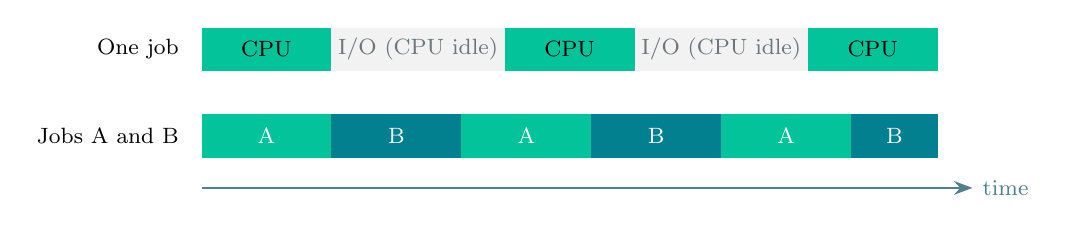
\begin{tikzpicture}[x=0.55cm,y=0.55cm,font=\footnotesize]
  % single program
  \node[anchor=east] at (-0.3,3.5) {One job};
  \foreach \a/\b/\c in {0/3/mint,3/7/light,7/10/mint,10/14/light,14/17/mint}
    \fill[\c] (\a,3) rectangle (\b,4);
  \node at (1.5,3.5) {CPU}; \node at (5,3.5) {\color{muted}I/O (CPU idle)}; \node at (8.5,3.5) {CPU};
  \node at (12,3.5) {\color{muted}I/O (CPU idle)}; \node at (15.5,3.5) {CPU};
  % multiprogramming
  \node[anchor=east] at (-0.3,1.5) {Jobs A and B};
  \foreach \a/\b/\c/\t in {0/3/mint/A,3/6/mintdeep/B,6/9/mint/A,9/12/mintdeep/B,12/15/mint/A,15/17/mintdeep/B}
    {\fill[\c] (\a,1) rectangle (\b,2); \node[text=white] at ({(\a+\b)/2},1.5) {\t};}
  \draw[-{Stealth},thick,color=slate] (0,0.3) -- (17.8,0.3) node[right] {time};
\end{tikzpicture}
\caption{Top: a single job leaves the CPU idle while it waits for I/O. Bottom: with two jobs in memory, the OS fills the gaps.}
\end{figure}

\begin{example}[A simple model of CPU utilization]
Suppose each job spends a fraction $p$ of its time waiting for I/O, and assume, for simplicity, that the jobs wait independently of each other. The CPU is idle only when \emph{all} $n$ jobs in memory are waiting at the same time, which happens with probability $p^{n}$. Therefore
\[
U(n) = 1 - p^{\,n}.
\]
For a typical I/O-heavy job with $p = 0.8$:
\[
U(1) = 1 - 0.8 = 20\%, \qquad U(4) = 1 - 0.8^{4} \approx 59\%, \qquad U(10) = 1 - 0.8^{10} \approx 89\%.
\]
More jobs in memory means a busier, more productive CPU. The model is simplified, since real jobs do not wait independently, but it shows why multiprogramming was worth the effort, and why \emph{memory} (Week~6) became so important: more memory means more jobs can be resident.
\end{example}

\begin{figure}[H]
\centering
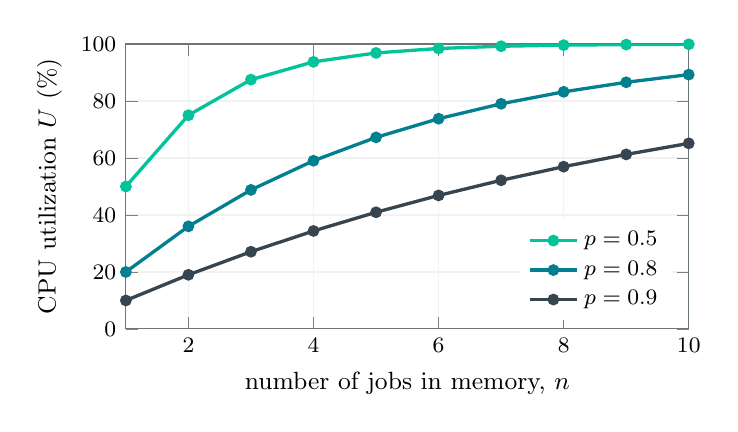
\begin{tikzpicture}
\begin{axis}[width=0.72\linewidth,height=5.2cm,xmin=1,xmax=10,ymin=0,ymax=100,
  xlabel={number of jobs in memory, $n$},ylabel={CPU utilization $U$ (\%)},
  grid=major,grid style={color=light},axis line style={color=muted},tick label style={font=\footnotesize},
  label style={font=\small},legend pos=south east,legend style={font=\footnotesize,draw=none,fill=white}]
\addplot[color=mint,very thick,mark=*,mark size=1.5pt,domain=1:10,samples=10] {100*(1-0.5^x)};
\addplot[color=mintdeep,very thick,mark=*,mark size=1.5pt,domain=1:10,samples=10] {100*(1-0.8^x)};
\addplot[color=charcoal,very thick,mark=*,mark size=1.5pt,domain=1:10,samples=10] {100*(1-0.9^x)};
\legend{$p=0.5$,$p=0.8$,$p=0.9$}
\end{axis}
\end{tikzpicture}
\caption{$U(n)=1-p^{n}$ for three different I/O-wait fractions $p$.}
\end{figure}

% ---------------------------------------------------------------------
\subsection{Time-sharing: many users, one machine, at once (1960s)}

Multiprogramming kept the CPU busy, but a programmer still submitted a job and waited hours for the result. \term{Time-sharing} solved this by connecting many \emph{terminals} (a keyboard plus a printer or screen) to one computer. The OS gives each user a small slice of CPU time, called a \term{time quantum}, in rapid rotation. Each user feels as if they have the whole machine.

The first successful demonstration was \textbf{CTSS} (Compatible Time-Sharing System) at MIT in 1961.

\begin{example}[Why it feels instant]
Suppose $n = 20$ users share one CPU and the OS gives each a quantum of $q = 10\ \text{ms}$. In the worst case a user waits for everybody else before running again:
\[
T_{\text{wait}} \approx n\,q = 20 \times 10\ \text{ms} = 200\ \text{ms}.
\]
A delay of about $0.2$\,s after pressing a key is barely noticeable to a human. The CPU is shared, but each user experiences an \emph{interactive} computer. With $n=200$ users, however, the wait grows to about $2$\,s, which is annoying. Choosing $q$ well is one of the scheduling questions of Weeks~4--5.
\end{example}

Time-sharing is the direct ancestor of every multi-user and multi-process system in use today, including your phone, which time-shares its CPU among dozens of apps and background services.

% ---------------------------------------------------------------------
\subsection{Multics: the giant that did not ship on time (1965--1969)}

In 1965, MIT, Bell Labs and General Electric started \term{Multics}, a time-sharing system meant to serve a whole city like a public utility: always on, easy to expand, and secure. Its ideas were far ahead of their time: hierarchical files and directories, dynamic memory management and fine-grained security. But the design was so ambitious that it grew slower and more expensive than planned, and Bell Labs withdrew in 1969. Multics did eventually run, but its most lasting effect was on two Bell Labs researchers who had worked on it.

% ---------------------------------------------------------------------
\subsection{UNIX is born (1969--1973)}

\begin{itemize}
  \item \textbf{1969.} Ken Thompson writes the first version of \term{UNIX} on a spare PDP-7 minicomputer at Bell Labs. It is deliberately small and simple, the opposite of Multics.
  \item \textbf{1970--1972.} Thompson and Dennis Ritchie grow it into a set of small, powerful tools that each do one job well and can be chained together.
  \item \textbf{1972--1973.} Ritchie designs the \textbf{C} programming language, and UNIX is rewritten in C. This is the single decision that lets UNIX later run on almost any hardware: to move it to a new machine, you mostly re-compile it, instead of re-writing it.
\end{itemize}

\begin{keyidea}[The UNIX philosophy (as summarized by Doug McIlroy)]
Write programs that do one thing and do it well. Write programs to work together. Write programs to handle text streams, because that is a universal interface.
\end{keyidea}

You will use this philosophy directly in Weeks~9--14. For example, the command
\begin{center}\cmd{cat access.log | grep "404" | wc -l}\end{center}
chains three tiny programs to count how many lines of a web-server log contain the error code 404.

Because UNIX was written in portable C and, for years, shared with universities, it did not stay one product; it split into a whole family: \textbf{BSD} (University of California, Berkeley, which added the TCP/IP networking the early Internet ran on), \textbf{HP-UX}, \textbf{AIX}, \textbf{SunOS/Solaris}, and later Apple's \textbf{macOS}, which is a certified UNIX.

% ---------------------------------------------------------------------
\subsection{The personal computer (1977--1995)}

\subsubsection{Apple II (1977)}
Designed by Steve Wozniak and sold by Apple Computer, the \term{Apple II} was one of the first successful mass-produced personal computers. It came with colour graphics and a built-in BASIC language, so it was ready to program the moment it was switched on. For the first time, the person using the computer and the person who owned it were usually the same person.

\subsubsection{The IBM PC and MS-DOS (1981)}

\begin{figure}[H]
\centering
\photo{0.5\linewidth}{5.5cm}{ibm_pc.png}
\caption{The IBM Personal Computer (model 5150), 1981.}
\label{fig:ibmpc}
\end{figure}

In 1981 IBM entered the market with the \term{IBM PC}, built quickly from off-the-shelf parts. Its operating system came from a small company called Microsoft, which had bought an existing system (86-DOS) and adapted it; IBM sold it as PC DOS, and Microsoft sold it to others as \term{MS-DOS}. MS-DOS was loaded from a floppy disk every time the machine started; a hard drive was not required.

IBM published detailed technical documentation for the PC. Once other companies, starting with Compaq, legally re-created the one piece IBM owned, the start-up firmware called the BIOS, they could build compatible ``clone'' machines. Thousands did, and ``PC compatible'' became the industry standard for the next twenty years.

\subsubsection{Graphical user interfaces}
\begin{itemize}
  \item \textbf{Xerox PARC, 1973.} Researchers build the \emph{Alto}, with overlapping windows, icons and a mouse. It was mostly a research machine and was never sold widely.
  \item \textbf{Apple Macintosh, 1984.} Brings these ideas to a mass-market product: point and click, a trash-can icon, a desktop metaphor, and no typed commands required.
  \item \textbf{Microsoft Windows, 1985--1995.} Starts as a graphical shell on top of MS-DOS; with \emph{Windows 95} it becomes the way most people use a PC.
\end{itemize}

For most users, typing commands stops being the norm. But the command line never disappears: it is still underneath, and it is where you will work in Weeks~9--14.

% ---------------------------------------------------------------------
\subsection{Linux is born (1991)}

\begin{histnote}[25 August 1991, a Usenet post]
``I'm doing a (free) operating system (just a hobby, won't be big and professional like gnu) for 386(486) AT clones.'' \hfill --- Linus Torvalds, a 21-year-old student in Helsinki
\end{histnote}

\term{Linux} is a new \emph{kernel} (the core of an operating system), written from scratch but deliberately compatible with UNIX in behaviour and commands. It contains no UNIX code; it is a ``UNIX-like'' system.

Two things made it spread:
\begin{itemize}
  \item \textbf{The licence.} From 1992 Linux was released under the \textbf{GNU General Public License (GPL)}: anyone may read, change and redistribute the source code, but modified versions must stay open too.
  \item \textbf{GNU.} Since 1983, Richard Stallman's \textbf{GNU Project} had been writing free versions of all the standard UNIX tools, except a kernel. Linux supplied the missing kernel. Together, GNU + Linux formed a complete, free operating system.
\end{itemize}

\subsubsection{Meanwhile, in the server room}
While Windows won the desktop, UNIX and Linux won the machines most people never see. They were built from the start for many simultaneous users and long uninterrupted uptime, and Linux is free to license, a decisive advantage once server farms grew to thousands of machines. Today Linux runs most web servers and cloud virtual machines, and since 2017 \emph{all} of the world's 500 fastest supercomputers (the TOP500 list).

% ---------------------------------------------------------------------
\subsection{Generation 6: the computer in your pocket (2007--2008)}

\begin{itemize}
  \item \textbf{iPhone (2007).} Apple's phone ran a full, modified version of its desktop operating system (what became iOS), not a stripped-down phone OS. It had a capacitive multi-touch screen for fingers, a real web browser, and, from 2008, an App Store. It proved that a modern multitasking OS could run on a battery-powered device.
  \item \textbf{Android (2008).} Android Inc.\ was founded in 2003 and bought by Google in 2005; the first Android phone (HTC Dream) shipped in 2008. Android's core is a \emph{modified Linux kernel}, and Google licenses it to any phone manufacturer for free. As a result, most smartphones on Earth are, underneath the app icons, running Linux.
\end{itemize}

% ---------------------------------------------------------------------
\subsection{Generation 7: the cloud (2006--today)}

Server hardware kept getting more powerful, but most programs did not need a whole physical machine to themselves.

\begin{itemize}
  \item \term{Virtualization.} A program called a \emph{hypervisor} lets one physical server pretend to be several independent computers (\emph{virtual machines}), each running its own guest operating system, isolated from the others.
  \item \term{Cloud computing.} From 2006, Amazon Web Services rented out virtual machines by the hour: you use someone else's data centre as if it were your own computer.
  \item \term{Containers.} An even lighter idea: instead of a whole guest OS, a container shares the host's Linux kernel and packages only the application and what it needs. Platforms such as Red Hat \emph{OpenShift} (2011) and Google's \emph{Kubernetes} (2014) run and manage thousands of containers across many machines.
\end{itemize}

Notice the pattern: a container is, at its core, a set of features of the Linux kernel that isolate processes from each other. Processes, memory protection and file systems, all topics of this course, are what the modern cloud is built on.

% ---------------------------------------------------------------------
\Needspace{12\baselineskip}
\subsection{The whole timeline at a glance}

\begin{center}
\small
\renewcommand{\arraystretch}{1.25}
\begin{longtable}{@{}p{1.9cm}p{4.3cm}p{8.4cm}@{}}
\toprule
\textbf{Year} & \textbf{Milestone} & \textbf{Why it matters for operating systems} \\
\midrule
\endhead
1837 & Analytical Engine (Babbage) & Processor (``mill'') + memory (``store'') + programs on cards \\
1843 & Lovelace's notes & First published computer program \\
1890 & Hollerith tabulator & Punch cards become the input medium for a century \\
1941 & Zuse Z3 & One of the first working programmable computers \\
1945 & ENIAC & Electronic, but no OS: one job, programmed by rewiring \\
1956 & GM-NAA I/O & Resident monitor, batch processing: the first OS \\
1961 & CTSS (MIT) & First time-sharing system: interactive computing \\
1964 & IBM System/360, OS/360 & One OS for a whole family of machines \\
1965--69 & Multics & Ambitious time-sharing; inspires UNIX \\
1969 & UNIX (Bell Labs) & Small, simple, composable tools \\
1973 & UNIX rewritten in C & Portable OS: runs on almost any hardware \\
1977 & Apple II & Personal computer for homes and schools \\
1981 & IBM PC, MS-DOS & PC-compatible standard; OS loaded from floppy \\
1983 & GNU Project & Free-software versions of UNIX tools \\
1984 & Apple Macintosh & Graphical interface for the mass market \\
1991 & Linux & Free UNIX-like kernel; with GNU, a complete free OS \\
1995 & Windows 95 & GUI becomes the default PC experience \\
2006 & Amazon Web Services & Cloud computing: rent virtual machines by the hour \\
2007 & iPhone & Full multitasking OS in a phone \\
2008 & Android & Linux kernel goes into billions of pockets \\
2011 / 2014 & OpenShift / Kubernetes & Containers managed at scale on Linux \\
\bottomrule
\end{longtable}
\end{center}

\begin{figure}[H]
\centering
\photo{\linewidth}{8cm}{timeline_infographic.png}
\caption{Timeline of operating systems, from GM-NAA I/O (1956) to OpenShift (2011).}
\label{fig:timeline}
\end{figure}

% =====================================================================
\section{Why This History Matters}

\begin{enumerate}[leftmargin=1.4em]
  \item \textbf{Every generation solved a real problem.} No OS $\to$ automation (batch) $\to$ sharing the CPU (multiprogramming) $\to$ sharing it interactively (time-sharing) $\to$ sharing it across the world (cloud). Every OS feature exists because someone was losing time or money without it.
  \item \textbf{Old ideas never really disappear.} Your phone still multiprograms, still time-shares, and still runs ``batch'' jobs in the background (backups, updates).
  \item \textbf{This course follows the same order.} We study processes, scheduling, memory and files roughly in the order they were invented to solve these problems.
\end{enumerate}

\begin{center}
\renewcommand{\arraystretch}{1.3}
\begin{tabularx}{\linewidth}{>{\raggedright\arraybackslash}p{5.2cm} >{\raggedright\arraybackslash}X}
\toprule
\textbf{Historical idea} & \textbf{Where you meet it again in MCMP117} \\
\midrule
Batch jobs waiting their turn & Weeks 3--4: process concept, process states \\
Multiprogramming and time-sharing & Weeks 4--5: CPU scheduling (FCFS, SJF, Priority, Round Robin) \\
Multics' memory and security ideas & Weeks 6--7: memory management, paging, virtual memory \\
Hierarchical files and directories & Week 7: file systems and directory structures \\
UNIX's small, composable tools & Weeks 9--14: Linux and Bash, full practical track \\
\bottomrule
\end{tabularx}
\end{center}

% =====================================================================
\section{Summary}

\begin{keyidea}[Week 1 in six sentences]
\begin{enumerate}[leftmargin=1.4em]
  \item A computer, at its core, follows instructions: input $\to$ process $\to$ output, with the program stored in memory.
  \item A first working definition: the OS is the program that starts first and manages everything else.
  \item We need an OS so that programs can safely share hardware, and so that programmers and users do not have to manage the hardware themselves.
  \item History moved from no software (ENIAC) $\to$ batch $\to$ multiprogramming/time-sharing $\to$ personal computers $\to$ mobile and cloud.
  \item Each step was driven by the cost of an idle processor, which we can estimate with simple formulas such as $U = \dfrac{t_{\text{run}}}{t_{\text{run}}+t_{\text{setup}}}$ and $U(n) = 1 - p^{n}$.
  \item Two dates worth remembering: UNIX, 1969; Linux, 1991, the system we will use hands-on later this semester.
\end{enumerate}
\end{keyidea}

% =====================================================================
\Needspace{12\baselineskip}
\section{Glossary}

\begin{description}[leftmargin=0pt,style=nextline,itemsep=0.2em]
  \item[Batch processing] Running a collected group of jobs one after another automatically, with no human interaction between them.
  \item[Kernel] The core part of an operating system, always in memory, that controls the hardware and manages resources.
  \item[Multiprogramming] Keeping several jobs in memory so the CPU can switch to another job while one waits for I/O.
  \item[Operating system (OS)] The program that starts first and manages the computer's hardware and all other programs.
  \item[Program] A list of instructions that tells the computer what to do.
  \item[Resident monitor] A small program kept permanently in memory that loads and starts jobs automatically; the earliest form of OS.
  \item[Stored-program computer] A computer that keeps its program in memory, like data, so it can be changed without rewiring.
  \item[System call] A request from a program to the operating system for a service (e.g.\ ``open this file'').
  \item[Time quantum] The small slice of CPU time the OS gives each program or user in turn.
  \item[Time-sharing] Switching the CPU among many interactive users so quickly that each feels they have the whole machine.
  \item[Utilization] The fraction of time a resource (usually the CPU) spends doing useful work.
  \item[Virtual machine] A software-created computer, running its own OS, on top of a real (physical) machine.
\end{description}

% =====================================================================
\Needspace{20\baselineskip}
\section{Try It Yourself}

\begin{tryit}[See multiprogramming on your own computer]
\textbf{Windows:} press \cmd{Ctrl+Shift+Esc} to open Task Manager and look at the \emph{Processes} tab. \textbf{Linux/macOS:} open a terminal and type \cmd{top} (press \cmd{q} to quit).
\begin{enumerate}[leftmargin=1.4em]
  \item How many processes are running right now? (Usually more than 100.)
  \item How many CPU cores does your computer have? (Task Manager $\to$ \emph{Performance}.)
  \item If there are far more processes than cores, how can they all be ``running''? Write two sentences using the words \emph{time-sharing} and \emph{multiprogramming}.
\end{enumerate}
\end{tryit}

% =====================================================================
\Needspace{12\baselineskip}
\section{Review Questions}

\subsection*{Conceptual}
\begin{enumerate}[leftmargin=1.6em]
  \item Draw the input--process--output model and give one example of each part for a smartphone camera.
  \item State the first working definition of an operating system and explain its three jobs in your own words.
  \item Give two problems that arise when there is no operating system and several programs want the same computer.
  \item Why is ENIAC described as a computer with ``no operating system at all''?
  \item What was a \emph{resident monitor}, and what problem did it solve?
  \item Explain the difference between \emph{multiprogramming} and \emph{time-sharing}. Which one is mainly about CPU efficiency, and which one is mainly about the user's experience?
  \item Why was rewriting UNIX in C in 1973 such an important decision?
  \item Linux contains no UNIX code. In what sense is it still a member of the UNIX family?
  \item Give one reason Linux won in servers even though Windows won on the desktop.
  \item How is a container different from a virtual machine?
\end{enumerate}

\subsection*{Numerical}
\begin{enumerate}[leftmargin=1.6em,resume]
  \item A job runs for $t_{\text{run}} = 3$ min and the operator needs $t_{\text{setup}} = 9$ min between jobs. Compute the CPU utilization. What must $t_{\text{setup}}$ become for $U = 90\%$?
  \item Jobs spend $p = 0.7$ of their time waiting for I/O. Using $U(n)=1-p^{n}$, find $U$ for $n = 1, 2, 5$. What is the smallest $n$ that gives $U \geq 95\%$?
  \item A time-sharing system has $n$ users and a quantum $q = 20$ ms. Users complain if they wait more than $0.5$ s. What is the largest number of users the system can support?
  \item A processor runs at $2.5$ GHz. How many clock cycles pass while it waits $5$ ms for a disk?
\end{enumerate}

\subsection*{Answers to the numerical questions}
\begin{enumerate}[leftmargin=1.6em,start=11]
  \item $U = \dfrac{3}{3+9} = 25\%$. For $U = 0.9$: $\dfrac{3}{3+t_{\text{setup}}} = 0.9 \Rightarrow t_{\text{setup}} = \dfrac{3}{0.9} - 3 \approx 0.33$ min $= 20$ s.
  \item $U(1) = 30\%$, $U(2) = 1 - 0.49 = 51\%$, $U(5) = 1 - 0.7^{5} \approx 83\%$. We need $0.7^{n} \leq 0.05$, i.e.\ $n \geq \dfrac{\ln 0.05}{\ln 0.7} \approx 8.4$, so $n = 9$.
  \item $n\,q \leq 0.5\ \text{s} \Rightarrow n \leq \dfrac{0.5}{0.020} = 25$ users. (Real systems also lose time switching between users, so the true limit is a little lower.)
  \item $N = f\,t = (2.5\times10^{9}\ \text{s}^{-1})(5\times10^{-3}\ \text{s}) = 1.25\times10^{7}$ cycles.
\end{enumerate}

% =====================================================================
\section{Looking Ahead: Week 2}

Next week we replace our informal definition with a precise one, and look inside the operating system:
\begin{itemize}
  \item a formal definition of an operating system, and its two classic views: \emph{resource manager} and \emph{extended machine};
  \item the design goals of an OS: convenience, efficiency and the ability to evolve;
  \item the four components of a computer system: hardware, operating system, application programs and users;
  \item how operating systems are built: monolithic, layered, microkernel and modular structures.
\end{itemize}

\subsection*{Further reading (optional)}
\begin{itemize}
  \item R.\,H.\ Arpaci-Dusseau and A.\,C.\ Arpaci-Dusseau, \emph{Operating Systems: Three Easy Pieces}, free online textbook: \url{https://pages.cs.wisc.edu/~remzi/OSTEP/}
  \item A.\ Silberschatz, P.\,B.\ Galvin and G.\ Gagne, \emph{Operating System Concepts}, 10th ed., Wiley, Chapter~1.
  \item A.\,S.\ Tanenbaum and H.\ Bos, \emph{Modern Operating Systems}, 4th ed., Pearson, Section~1.2 (``History of Operating Systems'').
  \item D.\,M.\ Ritchie, ``The Evolution of the Unix Time-sharing System'' (1979): \url{https://www.bell-labs.com/usr/dmr/www/hist.html}
\end{itemize}

\end{document}
